% !TeX root = ../main.tex
% Add the above to each chapter to make compiling the PDF easier in some editors.

\chapter{Experiments}\label{chapter:experiments}

\section{Datasets}
We train and test proposed method on three datasets. On the quantitative side, we use a synthetic CT vessel dataset and a real EM dataset. For qualitative comparison we use an MRA dataset of brain vessels.

\begin{itemize}
	\item \textbf{Synthetic CT Vessel (\cite{Tetteh2018}).} We use synthetic CT vessel dataset (\autoref{fig:intro} (b))for centerline detection task. The synthetic dataset consists of isotropic single-instance volumes of size $600\times304\times325$. We use 20 volumes for training and 15 for testing.
	
	\item \textbf{SNEMI3D (\cite{SNEMI3D}).} For neuron skeleton extraction, we conduct experiments on SNEMI3D (\autoref{fig:intro} (a)), a neuron segmentation benchmark for EM images containing packed and complex-shaped neuron instances. We create ground truth skeletons from segmentation by topological thinning~\cite{palagyi2014sequential}. The train volume is of size $100\times1024\times1024$ voxels with $30\times6\times6$ nm resolution. 
	As the test label is unavailable, we report results on a validation volume from the original paper ~\cite{Kasthuri2015}.
	
	\item  \textbf{Brain MRA (\cite{Bullitt2005}).} Brain MRA dataset (\autoref{fig:intro} (c)) consists of 42 volumes of annotated blood vessels of size $128\times448\times448$ and resolution $0.8\times0.5\times0.5$ mm. We use 28 volumes for training and show result on one test volume. We only show qualitative results because the ground truth skeletons were disconnected and therefore ground truth topology graph could not be created. Also, we found annotations missing for faintly identifiable vessels. 
\end{itemize}

\section{Evaluation Metric}
To evaluate multiple skeleton instances and their connectivity, we choose the {\em instance-level F1 score} , similar to \cite{Liang2019}. Each proposed skeleton is assigned to a single ground truth skeleton based on maximum overlap. All predicted skeleton voxels within a threshold distance to the mapped gt skeleton voxels are classified as true positives and rest as false positives. Ground truth voxels outside the range of predicted voxels are classified as false negatives. We also report mean {\em connectivity score (C)}, defined for each ground truth skeleton as $C_{i} = \frac{1(N_{i})}{N_{i}}$, where $N_{i}$ is the number of assigned predicted skeletons to ground truth $i$ and $1(\cdot)$ is the indicator function, similar to \cite{Liang2019}.
We also provide the {\em pixel-level F1 score} for semantic skeleton prediction as a sanity check.

\section{Methods in Comparison}
We compare our method with state-of-the-art deep learning based skeletonization methods defined as follows:
 
\begin{itemize}
	\item Predict {\em dilated binary mask}~\cite{cciccek20163d,Tetteh2018}.
	\item Predict {\em inverse truncated distance transform of skeletons}~\cite{wang2019deep}.
	\item {\em DeepFlux$^{\dagger}$}~\cite{Wang2019} extended from 2D skeleton cases.
	\item {\em Centerline Prediction}~\cite{sironi2015} (only for qualitative comparison on the MRA, results obtained from \cite{Koziski2018}).
\end{itemize}

We use the same U-net architecture and hyper-parameters for all methods. For each method we find the best thresholding parameter using grid search as shown in \autoref{tab:baseline_params}. We also dilate and erode the binarized predictions with kernel size of 3 and 4 respectively for all methods as done in the DeepFlux paper \cite{Wang2019}. We skip dilation for our Flux-and-Track method.

\begin{table}[t]
	\centering
	\begin{tabular}{l|cc}
		& \multicolumn{2}{c}{Thresholding Value}\\
		&~SNEMI~&~Synthetic CT~ \\
		\hline
		UNET-3D [5]           &  0.90 & 0.85\\
		DT [18]                 &  0.45 & 0.45\\
		DeepVesselNet [16]        &  -    & 0.30\\
		DeepFlux$^{\dagger}$ [19]   & 0.15  & 0.65\\
		Flux-and-Track (\textbf{Ours})         & 0.55  & 0.80 \\
		\hline
	\end{tabular}
	\caption{\label{tab:baseline_params}Table shows the threshold values used to binarize the prediction of different methods. We skip dilation for our Flux-and-Track method.}
\end{table}

\section{Results}

\subsection{Quantitative}

\begin{table}[htpb]
	% \yx{Duplicate references:~\cite{wang2019deep} and~\cite{YanWang2019}}.
	\centering
	\begin{tabular}{lccc|cc}
		& \multicolumn{3}{c}{SNEMI} & \multicolumn{2}{c}{Synthetic CT}\\
		\hline
		& ~F1-pix.~&~F1-ins.~&~C~&~F1-pix./F1-ins.~ \\\hline
		UNET-3D~\cite{cciccek20163d}           & \textbf{0.924}  & 0.695 & 0.625  & 0.833\\
		DT~\cite{wang2019deep}                 & 0.908  & 0.655 & 0.559  & \textbf{0.983}\\
		DeepVesselNet~\cite{Tetteh2018}        & -      & -     &  -     & 0.779\\
		DeepFlux$^{\dagger}$~\cite{Wang2019}   & 0.792  & 0.741 & 0.500  & 0.950\\\hline
		Flux-only (\textbf{Ours})              &    0.773   & 0.716 & 0.730  & 0.926\\
		Flux-and-Track (\textbf{Ours})  & 0.810 & \textbf{0.764} & \textbf{0.733} & - \\
		\hline
	\end{tabular}
	\caption{\label{tab:exp_em}Comparison on SNEMI and synthetic vessel dataset. DeepFlux$^{\dagger}$: extension of~\cite{Wang2019} to predict 3D skeletons instead of 2D.}
\end{table}

\begin{figure}[t]
	% \newcommand{\hwidth}{0.24\textwidth}
	\captionsetup[subfigure]{aboveskip=1pt, belowskip=1pt}
	\centering
	\begin{subfigure}[c]{0.15\textwidth}
		\frame{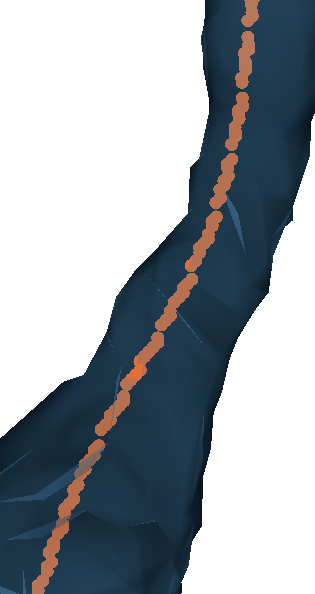
\includegraphics[width=\textwidth]{figures/final_results/gt.png}}
		\caption{\label{fig:final_results_a}}
	\end{subfigure}
	\null\hfill
	\begin{subfigure}[c]{0.15\textwidth}
		\frame{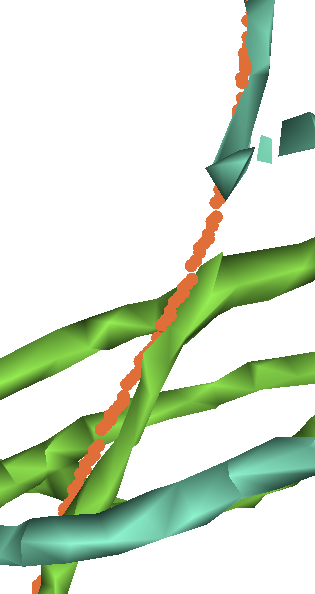
\includegraphics[width=\textwidth]{figures/final_results/dilated.png}}
		\caption{\label{fig:final_results_b}}
	\end{subfigure}
	\hfill
	\begin{subfigure}[c]{0.15\textwidth}
		\frame{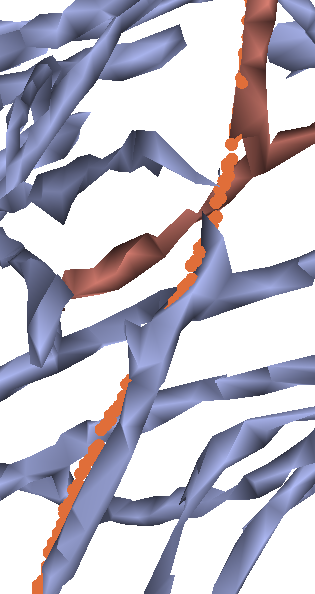
\includegraphics[width=\textwidth]{figures/final_results/distance_tx.png}}
		\caption{\label{fig:final_results_c}}
	\end{subfigure}
	\hfill
	\begin{subfigure}[c]{0.15\textwidth}
		\frame{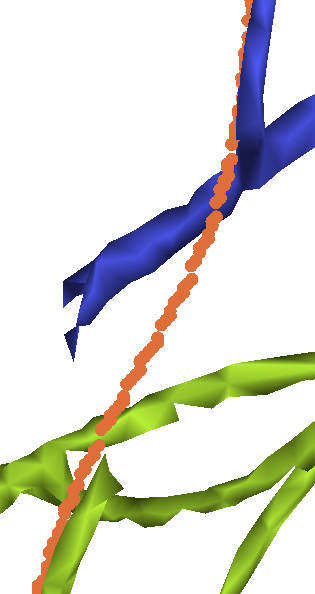
\includegraphics[width=\textwidth]{figures/final_results/deepflux.png}}
		\caption{\label{fig:final_results_d}}
	\end{subfigure}
	\begin{subfigure}[c]{0.15\textwidth}
		\frame{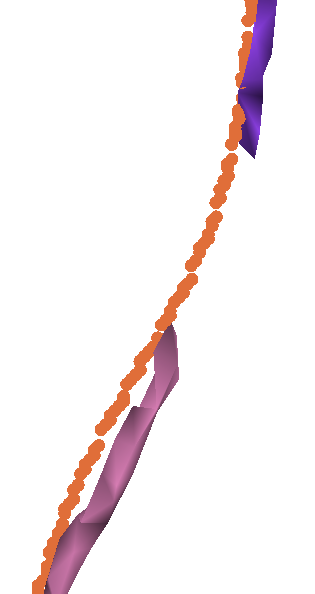
\includegraphics[width=\textwidth]{figures/final_results/ours_split.png}}
		\caption{\label{fig:final_results_e}}
	\end{subfigure}
	\begin{subfigure}[c]{0.15\textwidth}
		\frame{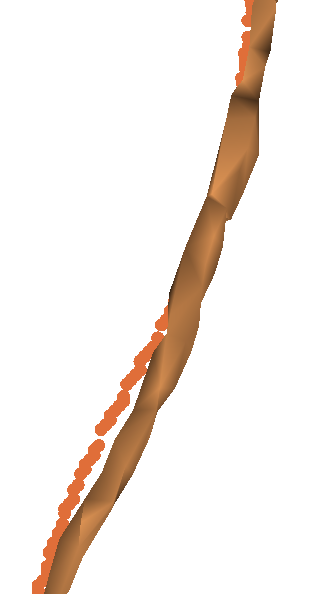
\includegraphics[width=\textwidth]{figures/final_results/ours.png}}
		\caption{\label{fig:final_results_f}}
	\end{subfigure}
	\hfill\null
	\caption{Qualitative results on SNEMI. (a) Ground Truth skeleton and segment (b) UNET-3D \cite{cciccek20163d} (c) DT \cite{wang2019deep} (d) DeepFlux$^{\dagger}$ \cite{Wang2019} (e) Our result after splitting (f) Our result after tracking }
	\label{fig:final_results}
\end{figure}

As shown in (\autoref{tab:exp_em}) our method outperforms other approaches for real dataset in {\em instance-level F1} and {\em connectivity} scores signifying that our method produces less instance false splits and merges. Other methods perform better on synthetic dataset because of its single instance and simple shapes. We do not run tracking on synthetic dataset as it has only a single instance, connectivity score is also not calculated therefore.
We show SNEMI3D qualitative results in \autoref{fig:final_results}. As can be noticed all other methods have severe false splits and merges, while our method performs better by learning more robust intermediate representations and utilizing topology information to resolve errors.

\subsection{Qualitative}

\begin{figure}[t]
	% \newcommand{\hwidth}{0.24\textwidth}
	\captionsetup[subfigure]{aboveskip=1pt, belowskip=1pt}
	\centering
	\begin{subfigure}[c]{0.24\textwidth}
		\frame{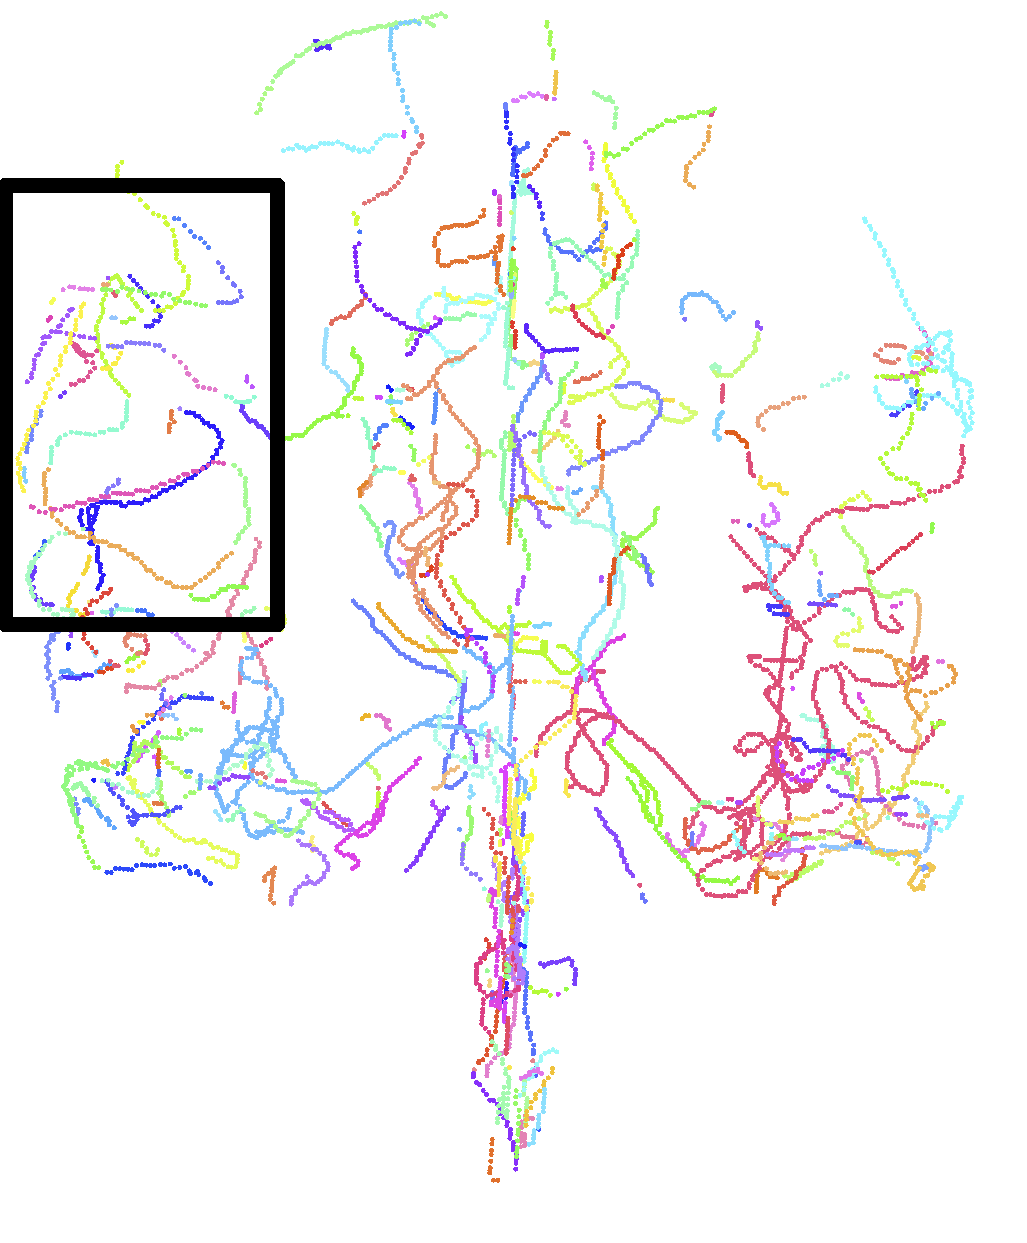
\includegraphics[width=\textwidth]{figures/mri_qualitative/gt_large.png}}
		\caption{\label{fig:mri_qual_a}}
	\end{subfigure}
	\begin{subfigure}[c]{0.18\textwidth}
		\frame{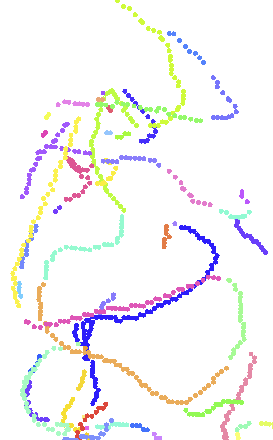
\includegraphics[width=\textwidth]{figures/mri_qualitative/gt.png}}
		\caption{\label{fig:mri_qual_b}}
	\end{subfigure}
	\null\hfill
	\begin{subfigure}[c]{0.18\textwidth}
		\frame{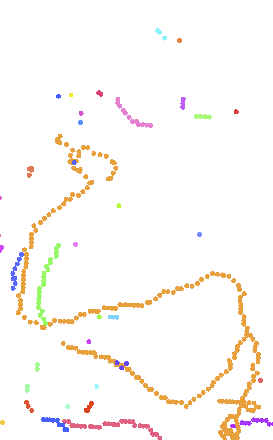
\includegraphics[width=\textwidth]{figures/mri_qualitative/sironi.png}}
		\caption{\label{fig:mri_qual_c}}
	\end{subfigure}
	\hfill
	\begin{subfigure}[c]{0.18\textwidth}
		\frame{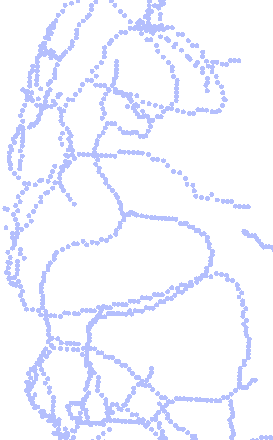
\includegraphics[width=\textwidth]{figures/mri_qualitative/dilated.png}}
		\caption{\label{fig:mri_qual_d}}
	\end{subfigure}
	\hfill
	\begin{subfigure}[c]{0.18\textwidth}
		\frame{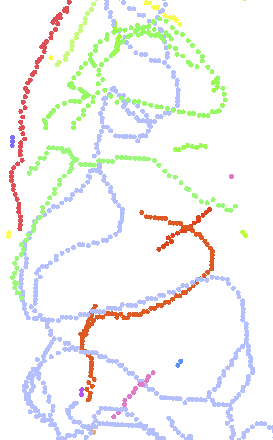
\includegraphics[width=\textwidth]{figures/mri_qualitative/ours.png}}
		\caption{\label{fig:mri_qual_e}}
	\end{subfigure}
	\hfill\null
	\caption{Qualitative MRA Results. (a) GT (b) Zoomed region from GT (c) Result from \cite{sironi2015} (d) Result from \cite{cciccek20163d} showing a false merge between disconnected vessels (e) Our result demarcates close vessels successfully.}
	\label{fig:mri_qualitative}
\end{figure}

We also visualized (\autoref{fig:mri_qualitative}) our results on the Brain MRA dataset\cite{Bullitt2005}, which has 42 volumes of annotated blood vessels of size $128\times448\times448$ and resolution $0.8\times0.5\times0.5$ mm. We use 28 volumes for training and show result of one test volume. We only show qualitative results because the ground truth skeletons were disconnected and also missing for many faint vessels. We compare our method with three other state-of-the-art methods in which Sironi \etall~\cite{sironi2015} doesn't manage to detect as many vessel instances as ours and a 3D Unet predicting binary output (UNET-3D)~\cite{cciccek20163d}. Although UNET-3D~\cite{cciccek20163d} can also perform effective detection in regions with artifacts, it fails to predict correct topology as shown in \autoref{fig:mri_qualitative} (d).

%\begin{figure}[htpb]
%	\centering
%	\begin{subfigure}[b]{0.3\textwidth}
%		\centering
%		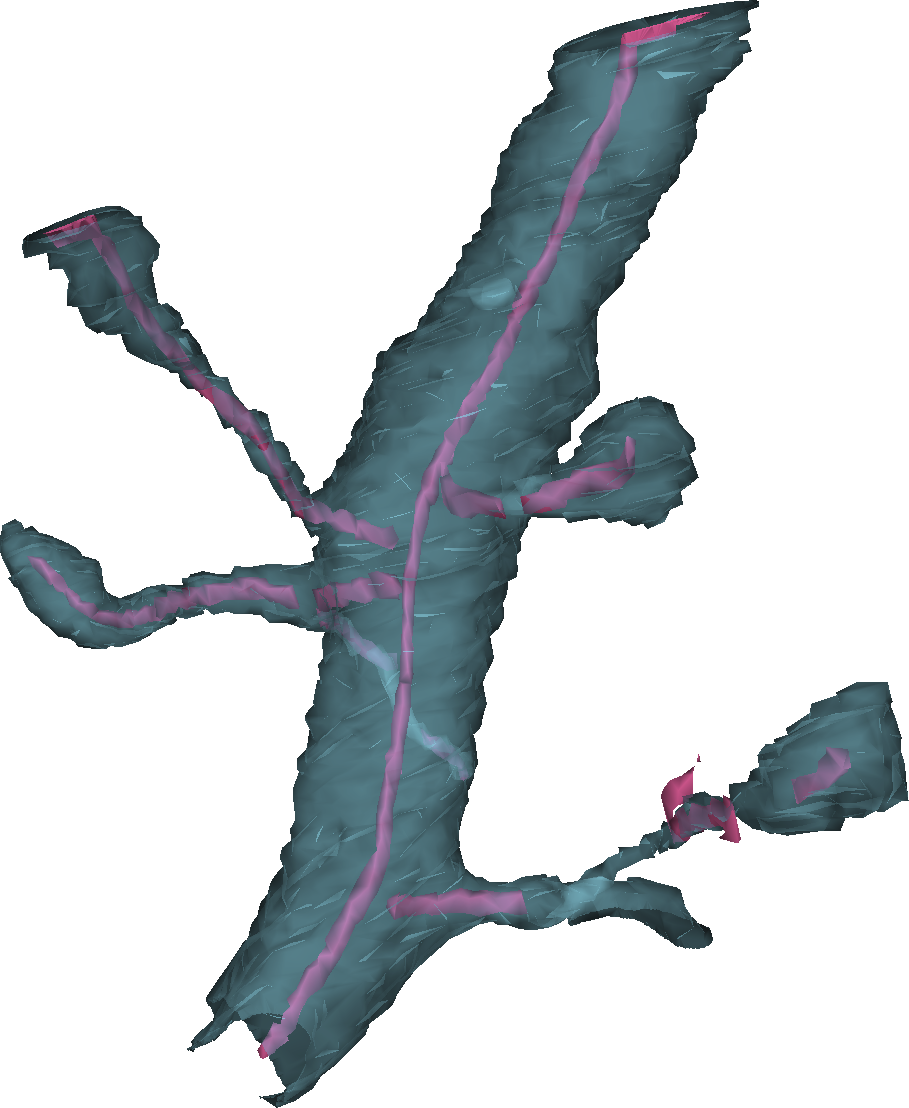
\includegraphics[width=\textwidth]{data/images/splitNMatch2/train_good.png}
%		\caption{\label{fig:merged_train}}
%	\end{subfigure}
%	\hspace{3mm}
%	\begin{subfigure}[b]{0.4\textwidth}
%		\centering
%		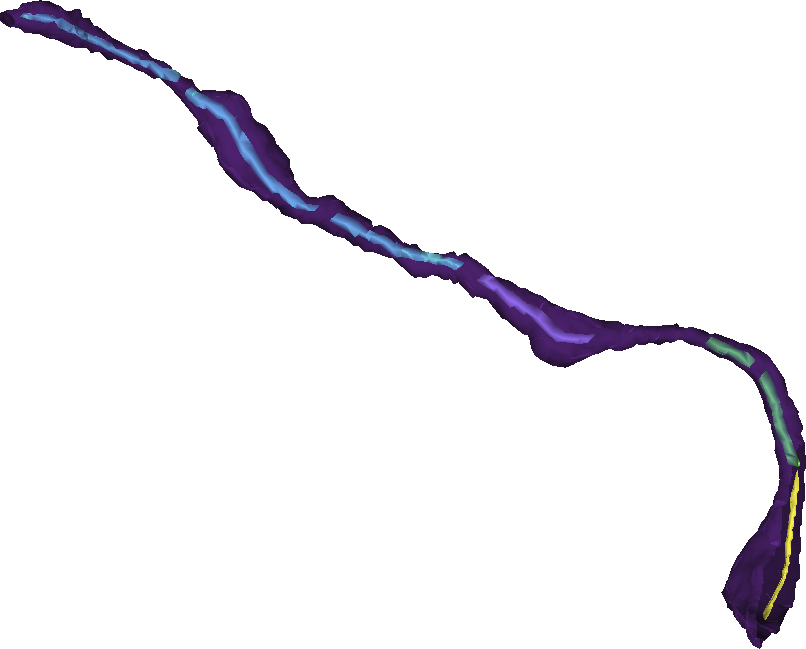
\includegraphics[width=\textwidth]{data/images/splitNMatch2/val_good_bad.png}
%		\caption{\label{fig:merged_val}}
%	\end{subfigure}	
%	\caption{Mathching results from \subref{fig:merged_train} train and \subref{fig:merged_val} test sets of SNEMI. While \subref{fig:merged_train} shows all the skeleton parts for a segment were matched properly, \subref{fig:merged_val} shows some correctly matched and some un-matched parts}  
%	\label{fig:matchedSNEMI}
%\end{figure}
%
%\begin{table*}[!ht]                                                                                          
%	\centering
%	\begin{adjustbox}{width=\textwidth,center=\textwidth}
%	\begin{tabular}{|c|c|c|c|c|c|c|c|c|c|c|c|c|c|}                                                                      
%		\hline                                                                                               
%		\multirow{2}{*}{Dataset} & \multirow{2}{*}{Subset} & \multicolumn{4}{c|}{Initial}  & \multicolumn{4}{c|}{After split}  & \multicolumn{4}{c|}{After match} \\                                    
%		\cline{3-14}                                                                                                  
%		&  & P & R & F & C & P & R & F & C & P & R & F & C \\                                                           
%		\hline                                                                                                  
%		\hline                                                                                                  
%				& Train & 0.64 & 0.89 & 0.74 & 0.93 & 0.66 & 0.96 & 0.78 & 0.74 & 0.66 & 0.95 & 0.78  & 0.79\\                           
%		SNEMI 	& Val 	& 0.64 & 0.64 & 0.64 & 0.88 & 0.63 & 0.82 & 0.71 & 0.73 & 0.62 & 0.76 & 0.68 & 0.77 \\           
%				& Test 	&  &  &  &  &  &  &  &  &  &  &  & \\
%		\hline		 
%				& Train &  &  &  &  &  &  &  &  &  &  &  & \\                           
%		P7 		& Val 	&  &  &  &  &  &  &  &  &  &  &  & \\           
%				& Test 	&  &  &  &  &  &  &  &  &  &  &  & \\                          
%		\hline                                                                                                     
%	\end{tabular}
%	\end{adjustbox}                                                
%	\caption{Skeleton prediction scores after every step. P, R, F, C stands for Precision, Recall, F-Score and Connectivity Scores.}
%	\label{tab:dissected_scores}                                                                   
%\end{table*}
